\documentclass{article}
\usepackage{amssymb}
\usepackage{graphicx} 
\usepackage{amsmath}
\usepackage{amsfonts}
\usepackage[a4paper, left=2cm, right=2cm, top=2cm, bottom=2cm]{geometry}

\title{Lista 2 Fundamentos Matemáticos da Computação II - Respostas}
\author{Alesandro Alex Mendes da Silva\\
        Francisco Matheus Fonseca de Farias\\
        Ryan David dos Santos Silvestre\\
        Sávio Emanuel Mariano Fonseca\\
        Sebastião Fellipe Pinto Lopes\\
        Weuller dos Santos Barbosa}

\begin{document}

\maketitle

\section{Seção Múltipla Escolha}

\subsection{Questão M1} 
Como $A = \{x \in \mathbb{Z} | 1 \leq x \leq 3\}$ e $B = \{y \in \mathbb{Z} | y \text{ é par e } 0 \leq y \leq 2\}$, logo $A = \{1,2,3\}$ e $B = \{0,2\}$ e o produto cartesiano será:

\[
    A \times B = \{(1,0),(1,2),(2,0),(2,2),(3,0),(3,2)\}
\]

Dessa forma, a alternativa correta é a letra \textbf{C}


\subsection{Questão M2}
Dado \( A = \{0, 1, 2, 3, 4\} \), \( B = \{0, 1, 2, 3\} \) e a relação \( R = \{(a, b) \in A \times B \mid a \mid b\} \), determinamos os pares \((a, b)\) em que \(a\) divide \(b\):

\[
R = \{(1, 0), (1, 1), (1, 2), (1, 3), (2, 0), (2, 2), (3, 0), (3, 3), (4, 0)\}.
\]

Portanto, a alternativa correta é \textbf{A}.
\subsection{Questão M3}
Seja \( A \) um conjunto com cardinalidade \( |A| = 4 \) e \( B \) um conjunto com cardinalidade \( |B| = 3 \). A quantidade de relações binárias distintas entre \( A \) e \( B \) pode ser determinada da seguinte forma:

Uma relação binária entre \( A \) e \( B \) é um subconjunto do produto cartesiano \( A \times B \). O número de elementos do produto cartesiano \( A \times B \) é dado por:

\[
|A \times B| = |A| \times |B| = 4 \times 3 = 12
\]

Agora, como cada elemento de \( A \times B \) pode ser incluído ou não em uma relação, o número total de relações binárias (subconjuntos) s é dado por:

\[
\text{Número de relações binárias} = 2^{12}
\]

Portanto, a alternativa correta é a letra \textbf{B}
\subsection{Questão M4}

Considerando as definições de Injetividade, Sobrejetividade e Bijetividade, a resposta correta é a letra \textbf{E (i) bijetora (ii) injetora (iii) sobrejetora}


\vspace{0.5em}
\hrule
\vspace{0.5em}

\section{Seção Discursiva}

\subsection{Questão D1}
Seja o conjunto \( A = \{1, 2, 3, 4\} \) e a relação \( R \subseteq A \times A \) definida por:
\[
R = \{(1, 1), (1, 2), (2, 1), (2, 2), (3, 3), (4, 4)\}.
\]

Analisemos as propriedades da relação \(R\):

\begin{enumerate}
    \item \textbf{Reflexiva:}  
    A relação \(R\) é reflexiva se, para todo \(a \in A\), \((a, a) \in R\).  
    Como \(R\) contém \((1, 1), (2, 2), (3, 3)\) e \((4, 4)\), a relação \(R\) é \textbf{reflexiva}.

    \item \textbf{Simétrica:}  
    A relação \(R\) é simétrica se, para todo \((a, b) \in R\), também \((b, a) \in R\).  
    Como \((1, 2) \in R\) e \((2, 1) \in R\), e não há outros pares que violem a simetria, a relação \(R\) é \textbf{simétrica}.

    \item \textbf{Anti-simétrica:}  
    A relação \(R\) é anti-simétrica se, para todo \((a, b) \in R\) e \((b, a) \in R\), temos \(a = b\).  
    Como \((1, 2) \in R\) e \((2, 1) \in R\) com \(1 \neq 2\), a relação \(R\) não é \textbf{anti-simétrica}.

    \item \textbf{Transitiva:}  
    A relação \(R\) é transitiva se, para todo \((a, b) \in R\) e \((b, c) \in R\), também \((a, c) \in R\).  
    Não há casos que violem a transitividade, logo \(R\) é \textbf{transitiva}.

    \item \textbf{Classificação:}  
    Como \(R\) é reflexiva, simétrica e transitiva, ela pode ser classificada como uma relação de \textbf{equivalência}.
\end{enumerate}
\subsection{Questão D2}
% SUA RESPOSTA DA D2
\begin{figure}[h]
    \centering
    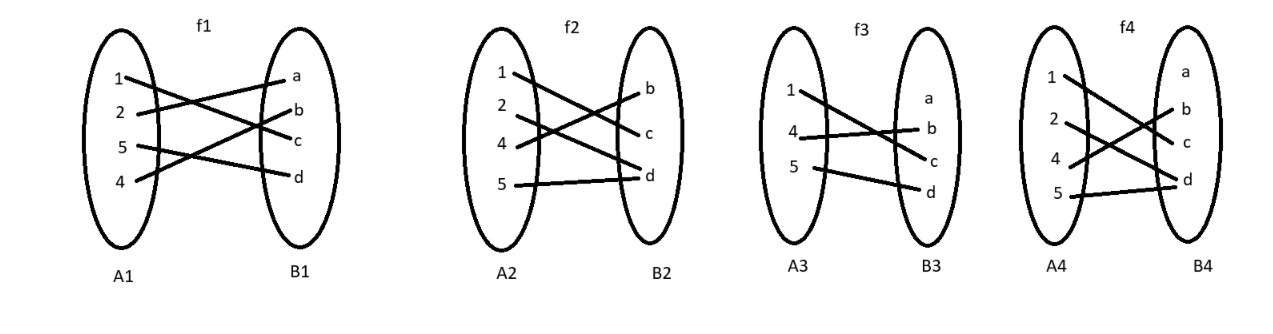
\includegraphics[width=1\textwidth]{qd2.png} 
    \label{fig:questaoD2}
\end{figure}

Dada a relação entre os conjuntos \(A\) e \(B\) para as funções \(f_1, f_2, f_3, f_4\), analisamos se são injetoras, sobrejetoras ou bijetoras:

\begin{itemize}
    \item \textbf{\(f_1\):}
    \begin{itemize}
        \item Cada elemento de \(A1\) tem uma correspondência distinta em \(B1\). Todos os elementos de \(B1\) são atingidos.
        \item \textbf{Conclusão:} \(f_1\) é \textbf{bijetora} (injetora e sobrejetora).
    \end{itemize}
    \item \textbf{\(f_2\):}
    \begin{itemize}
        \item Nem todos os elementos de \(A2\) possuem imagens distintas (\(2\) e \(5\) têm a mesma imagem em \(B3\)). Nem todos os elementos de \(B2\) são atingidos (\(a\) não é imagem de nenhum elemento de \(A2\)).
        \item \textbf{Conclusão:} \(f_2\) é \textbf{sobrejetora}.
    \end{itemize}
    \item \textbf{\(f_3\):}
    \begin{itemize}
        \item Cada elemento de \(A3\) tem uma correspondência distinta em \(B3\). Nem todos os elementos de \(B3\) são atingidos.
        \item \textbf{Conclusão:} \(f_3\) é \textbf{injetora}.
    \end{itemize}
    \item \textbf{\(f_4\):}
    \begin{itemize}
        \item Nem todos os elementos de \(A4\) possuem imagens distintas (\(2\) e \(5\) têm a mesma imagem em \(B4\)). Nem todos os elementos de \(B4\) são atingidos (\(a\) não é imagem de nenhum elemento de \(A4\)).
        \item \textbf{Conclusão:} \(f_4\) é \textbf{nenhum}.
    \end{itemize}
\end{itemize}

\end{document}
